\chapter{Technical Description}\label{ch:technical_description}
As afore-mentioned Quantum computing can help machine learning in two ways- data and computation. Based on this Quantum Machine Learning can be divided into 3 approaches.
\begin{enumerate}
\item Quantum enhanced Machine Learning ( classical data with quantum algorithms) 
\item Classical learning applied to quantum systems ( classical algorithm with quantum data)
\item Fully quantum machine learning (both data and algorithm is quantum based)
\end{enumerate}
\begin{figure}[H]
\centering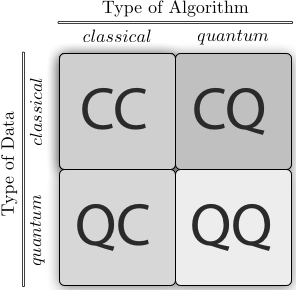
\includegraphics[width=.3\textwidth]{images/approach.png}
\caption{Approaches in Quantum Machine Learning}
\end{figure}
\section{Quantum Enhanced Machine Learning}
Quantum Enhanced Machine Learning is the most promising of these methods on early quantum computers. Such algorithms typically require one to encode the given classical dataset into a quantum computer, so as to make it accessible for quantum information processing. Machine learning techniques use mathematical algorithms and tools to search for patterns in data. The most important and time taking parts of machine learning algorithms are searching, sampling, optimization. We explain how these can be improved by Quantum Computing in the following sections.
\section{Search: Grover's algorithm}
when you compute Grover's Algorithm your are simultaneously testing every input value to see which is the correct input value. Using quantum superposition you can get qubits in a state that represents all possible inputs. Then run that superposition of states through some function to get each input together with its associated output. You are given a list of $n$ elements, and you know that one element satisfies a certain condition, while the other n-1 elements don't. Basically, this is an algorithm for finding a specific element in an unordered list. A classical computer would not be able to exploit any structure in this problem and therefore needs to scan up to $n-1$ elements to find the one needed.
Prepare $n$ qubits in a uniform state so that all $2^n$ numbers are in a uniform superposition, each with a coefficient of $1/\sqrt{n}$ If we would measure the $n$ qubits now, all $2^n$ results would be equally likely.\\
Then run the Grover iteration $k$ times, which consists of two steps (which can be merged into 1 step):
\begin{enumerate}
\item Negate the coefficient of the sought element. This is a unitary operation, which leaves all elements not satisfying the condition as they are and only negates the intended one.
\item Reflect all quantum states at the arithmetic mean of all quantum states. This also is a unitary operation.
\end{enumerate}
Each iteration amplifies the coefficient of the correct solution while damping the coefficient of all $n-1$ incorrect solutions, however only to a certain point.
If you choose the number of iterations $k$ correctly, you have maximized the coefficient for the correct solution. This means that the sought element's probability is now (almost) 1, so if we measure the qubits, we are very likely to get the correct answer. If we don't get it, we can repeat the algorithm from the beginning until we get the right answer. Doing more or less than the optimal $k$ iterations reduces the probability of finding the correct solution - however, the algorithm periodically reaches the maximum coefficient.
It can be shown that $k=O(\sqrt{n})$ This is remarkable, because a classical computer needs $O(n)$ steps for solving this problem. This is only a quadratic speedup (rather than an exponential speedup as for other quantum algorithms), but the Grover algorithm has quite a large number of useful applications and is fairly simple.
The Grover algorithm can be extended to support a predefined number of $m (0\leq m\leq n)$ elements which satisfy the condition, instead of 1. m need not be known in advance. Quantum period finding can be used to determine m before starting the extended Grover algorithm.
\begin{figure}[H]
\centering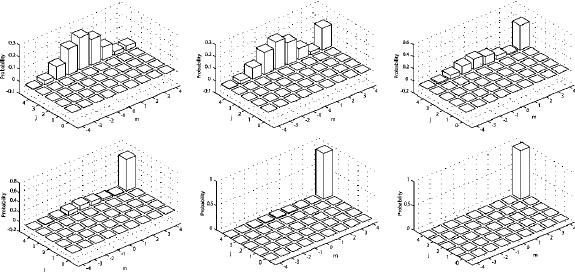
\includegraphics[width=1\textwidth]{images/grover.png}
\caption{Grover's Search}
\end{figure}

